\section{Disk Arrangements}
It turns out the disk arrangements are an equivalent way to to represent linkages and their corresponding problems.  Before we establish the relation, we will cover some fundamental concepts of disk arrangements.  
A \it{disk arrangement} is a set, $\DD$, is pairwise interior-disjoint disks in the plane.
%A \it{disk arrangement}, $P$, embedded in a plane  is a set of disks with disjoint interiors $\left\lbrace C_i \right\rbrace_{i = 1}^n $ such that for any circle $C \in \left\lbrace C_i \right\rbrace_{i = 1}^n$, $C$ is tangent to a different circle of $\left\lbrace C_i \right\rbrace_{i = 1}^n$. 
\begin{thm}[Disk Packing Theorem]\label{thm2-1}
For every connected simple planar graph $G$ there is a disk arrangement in the
plane whose intersection graph is (isomorphic to) $G$.
\end{thm}
\begin{figure}[h]
\begin{center}
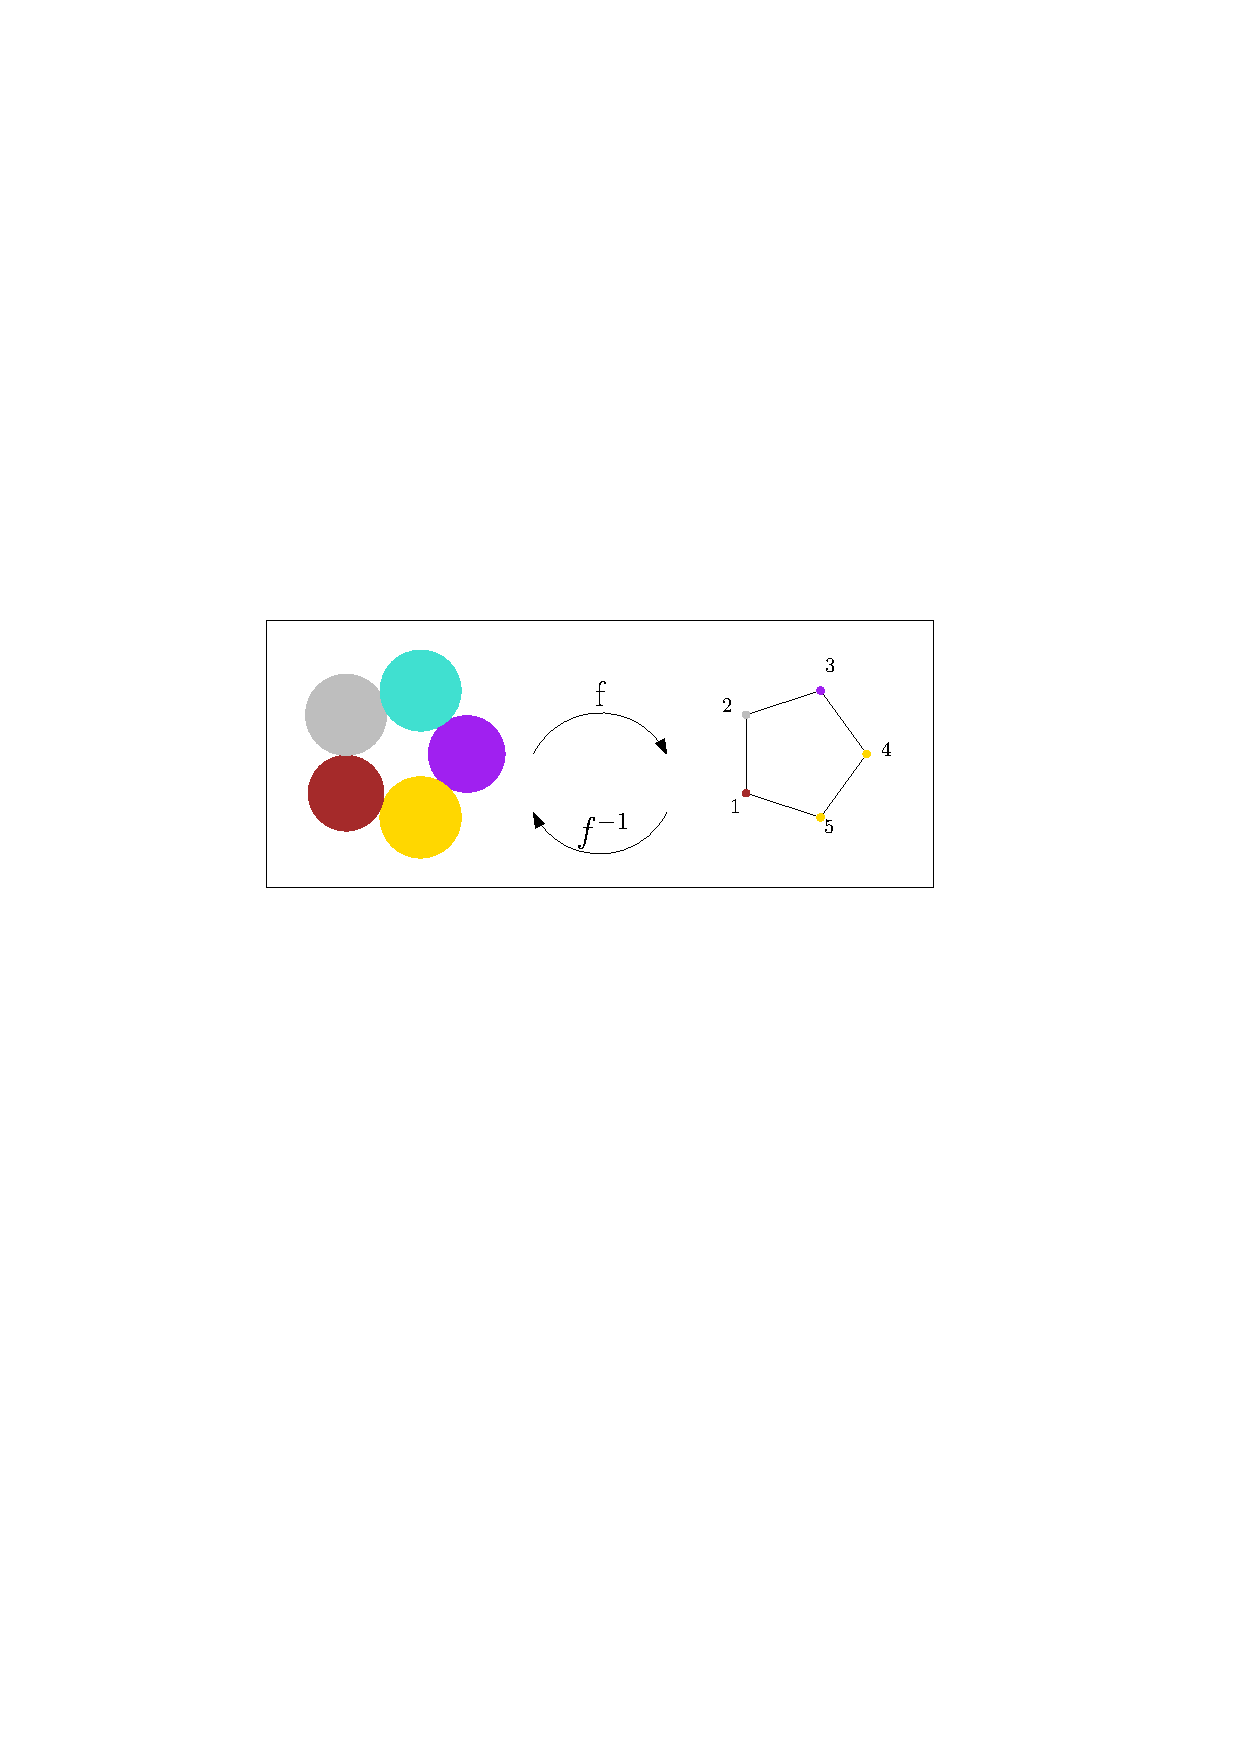
\includegraphics[scale=1]{graphics/diskPackingTheoremExample.pdf}
\end{center} 
\caption{This example represents a disk arrangement transformed to and from its corresponding graph 
$G_2$}
\label{fig:DiskArrangement-1}
\end{figure}
\begin{enumerate}%1,2,3,4....
%\item Introduce the circle packing theorem.
\item Show the relation between polygonal linkages and disk arrangengements.
\end{enumerate} 
\subsection{Oriented Realizations}
\begin{itemize}
\item[\rn{1}]have the professor explain this part.
\end{itemize}  
\subsection{Disk Packing Confinement Problem}
Consider the iterative problem:
\begin{enumerate}%1,2,3,4....
\item Start with a circle of diameter 1.
\item Add two kissing circles, each of diameter 1, that do not intersect with any other circle (they may kiss other
circles).
\item For each new kissing circle added, add two more non-intersecting kissing circles to it.
\end{enumerate} 
Figure (\ref{fig:circlePacking-1}) illustrates the iterative problem.  The problem with this is that the area in
which is necessary to contain this disk growing disk arrangement will exceed the area needed to contain it.
\begin{figure}[h]
\begin{center}
    %add desired spacing between images, e. g. ~, \quad, \qquad etc.
    %(or a blank line to force the subfigure onto a new line)
  \begin{subfigure}[b]{0.24\textwidth}
	  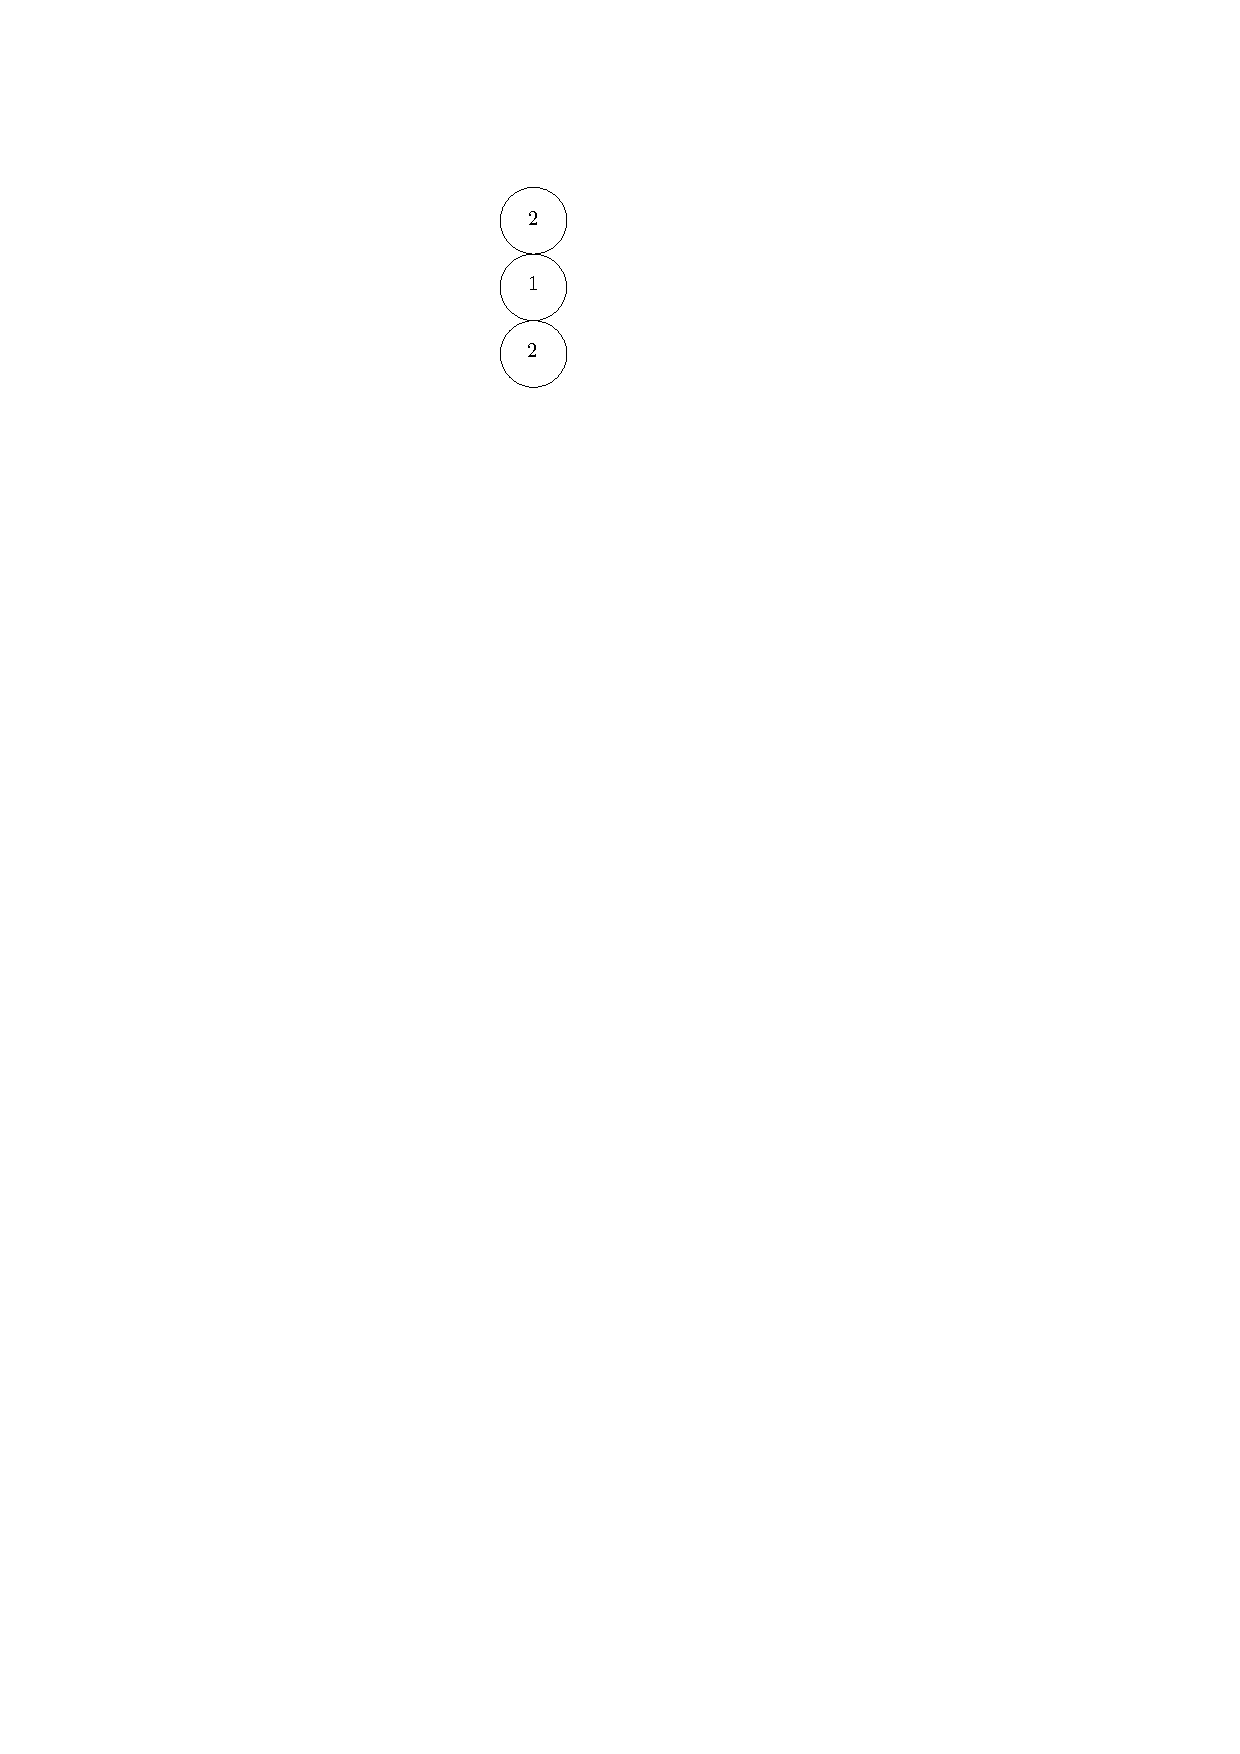
\includegraphics[width=\textwidth]{graphics/degree2arrangement.pdf}
	  \caption{A disk arrangement with two layers of disks}
	  \label{fig:circlePacking1-1}
  \end{subfigure}
  \begin{subfigure}[b]{0.24\textwidth}
	  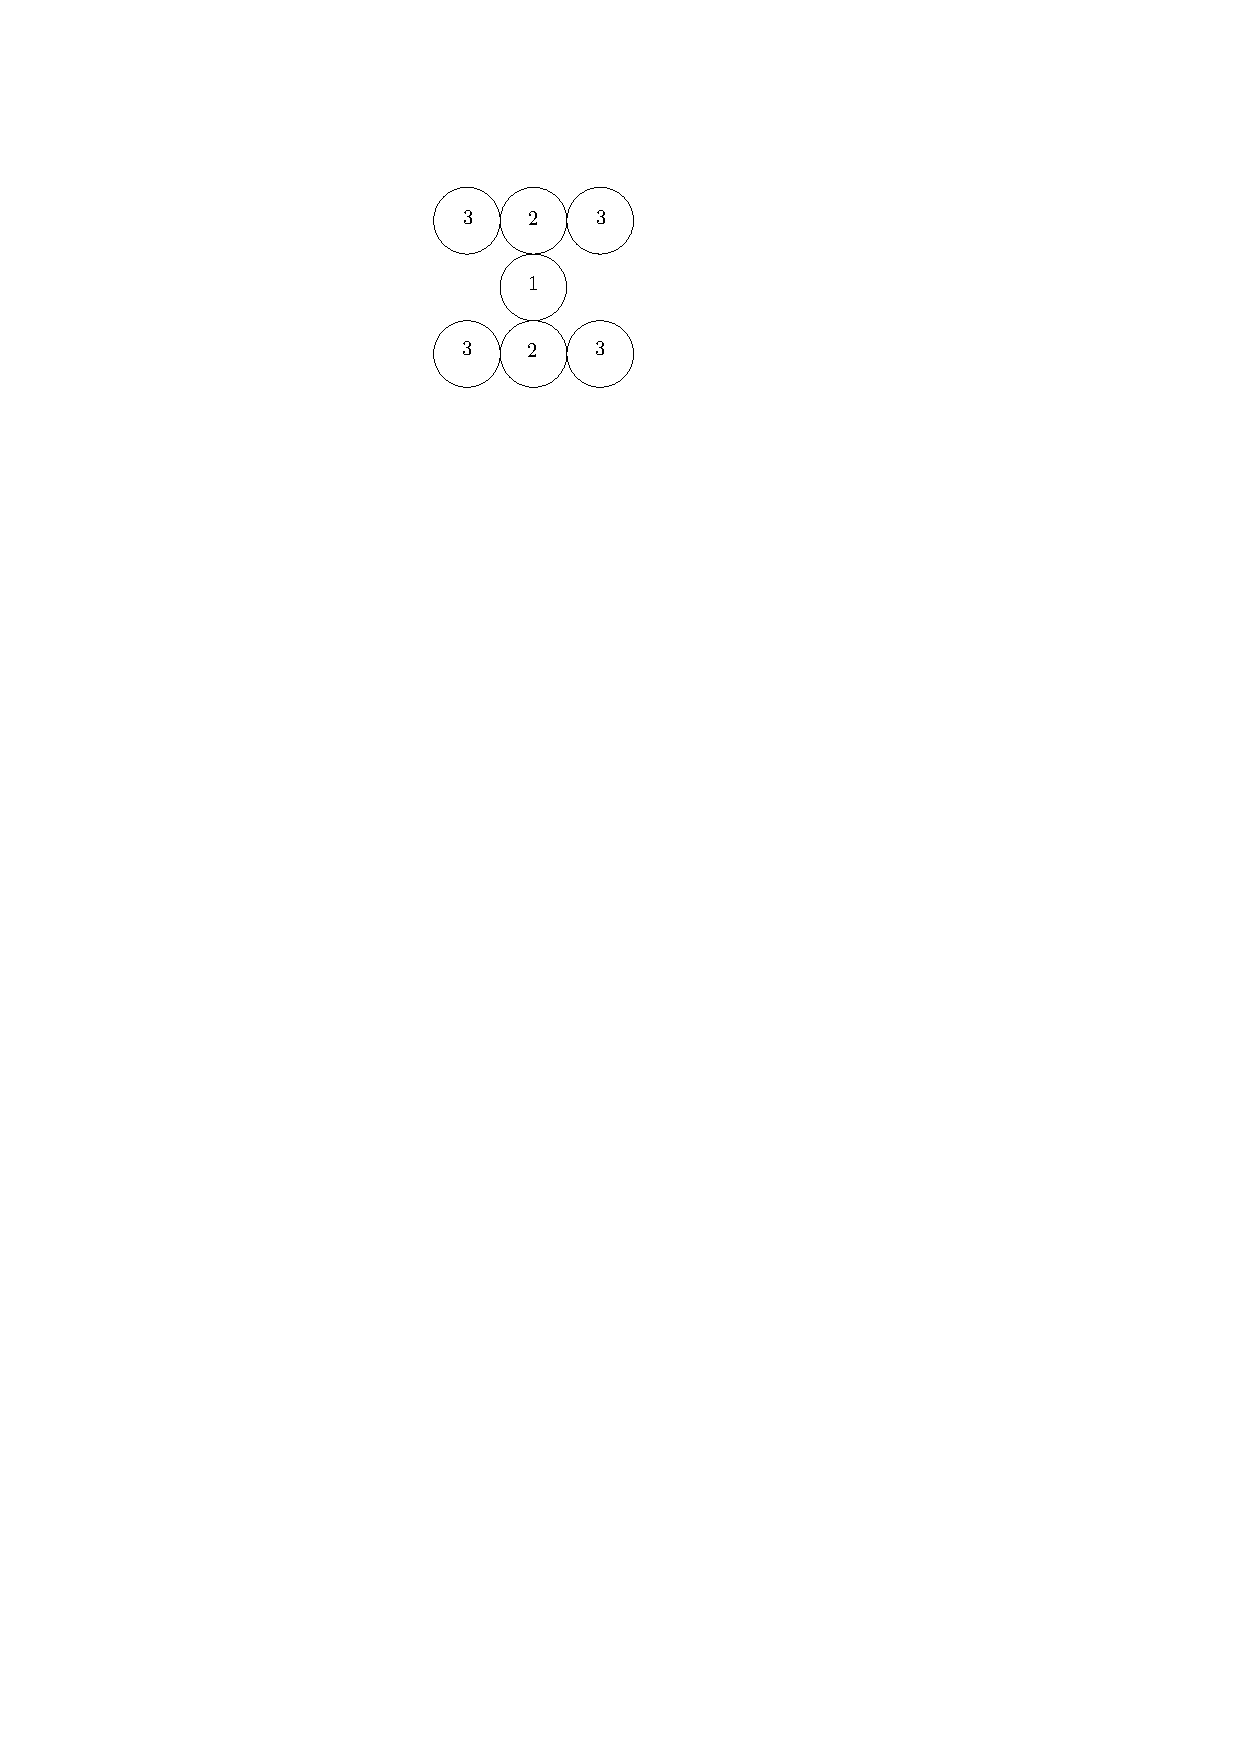
\includegraphics[width=\textwidth]{graphics/degree3arrangement.pdf}
	  \caption{A disk arrangement with three layers of disks}
	  \label{fig:circlePacking1-2}
  \end{subfigure}
  \begin{subfigure}[b]{0.24\textwidth}
	  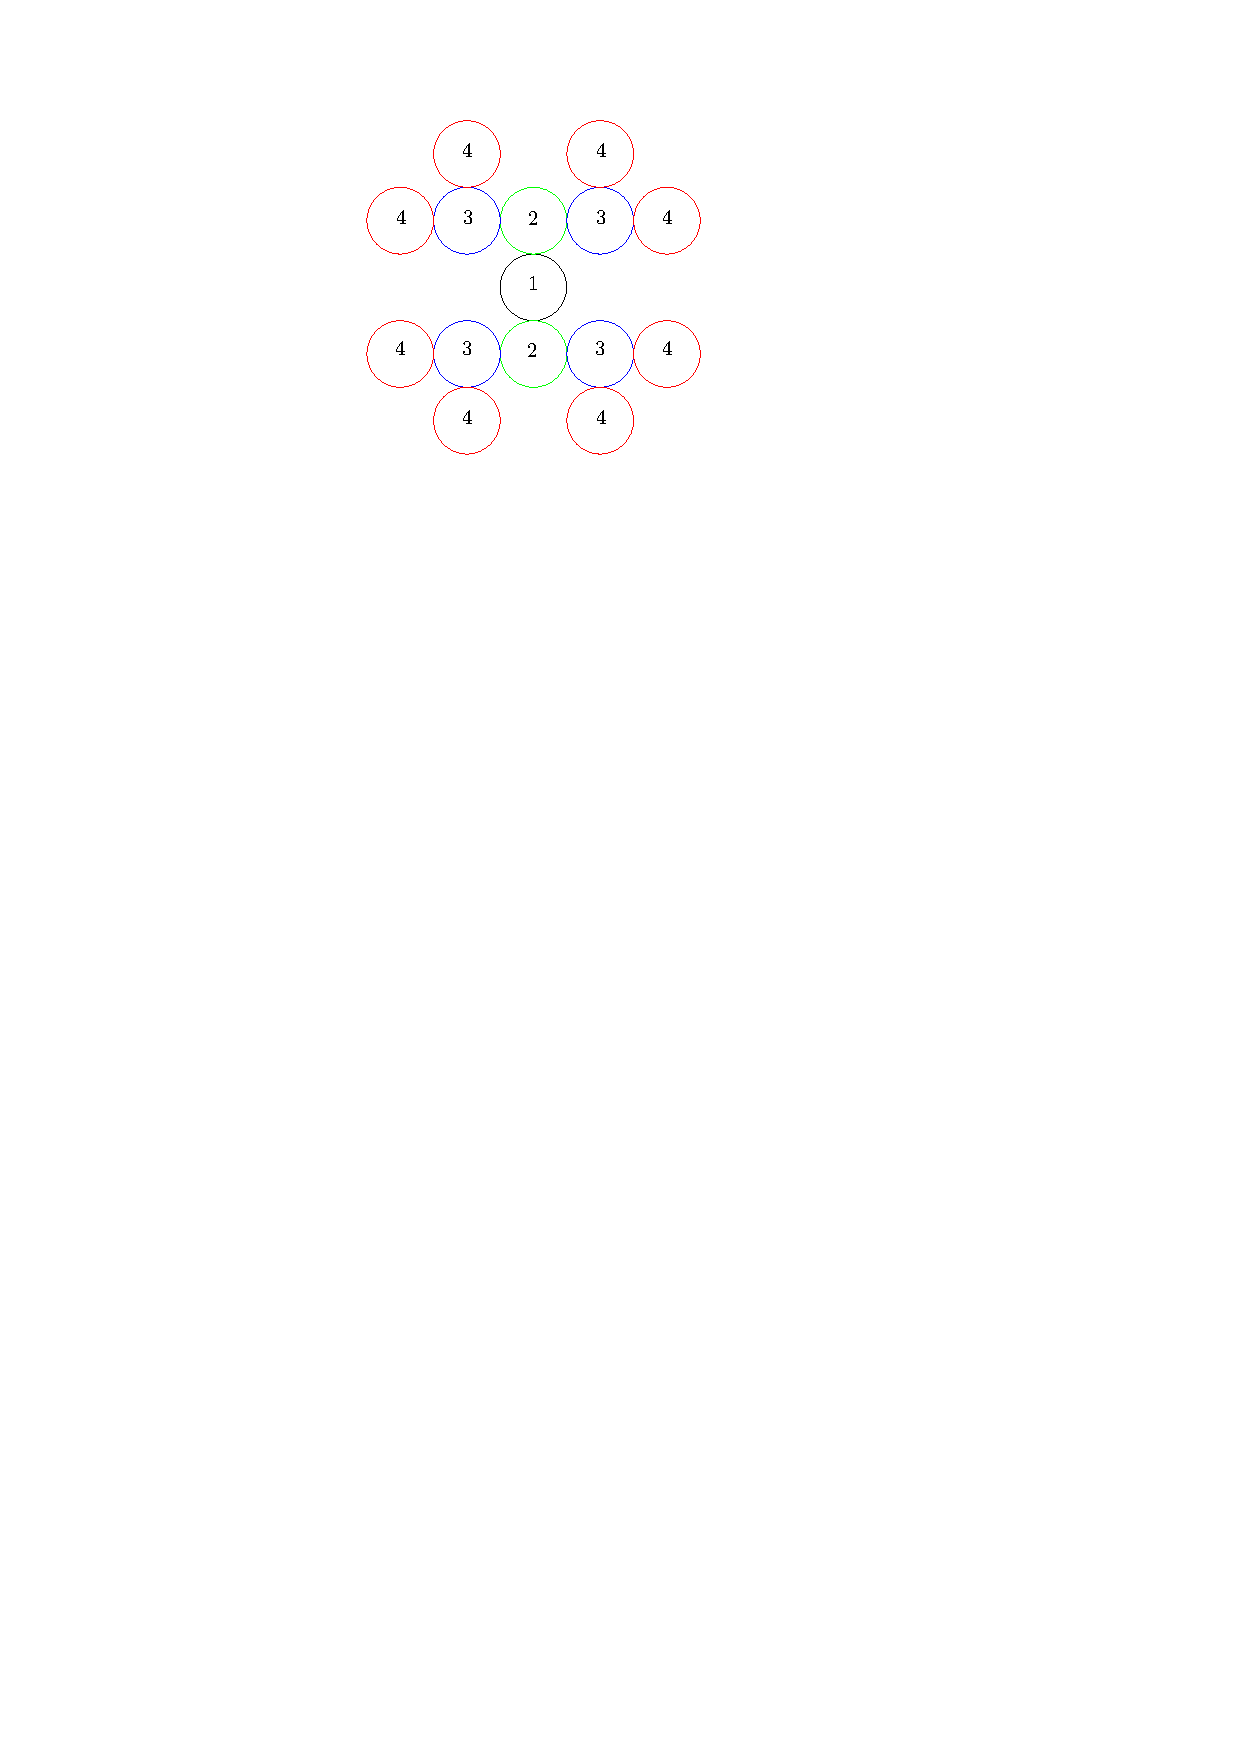
\includegraphics[width=\textwidth]{graphics/degree4arrangement.pdf}
	  \caption{A disk arrangement with four layers of disks}
	  \label{fig:circlePacking1-3}
  \end{subfigure}
  \begin{subfigure}[b]{0.24\textwidth}
	  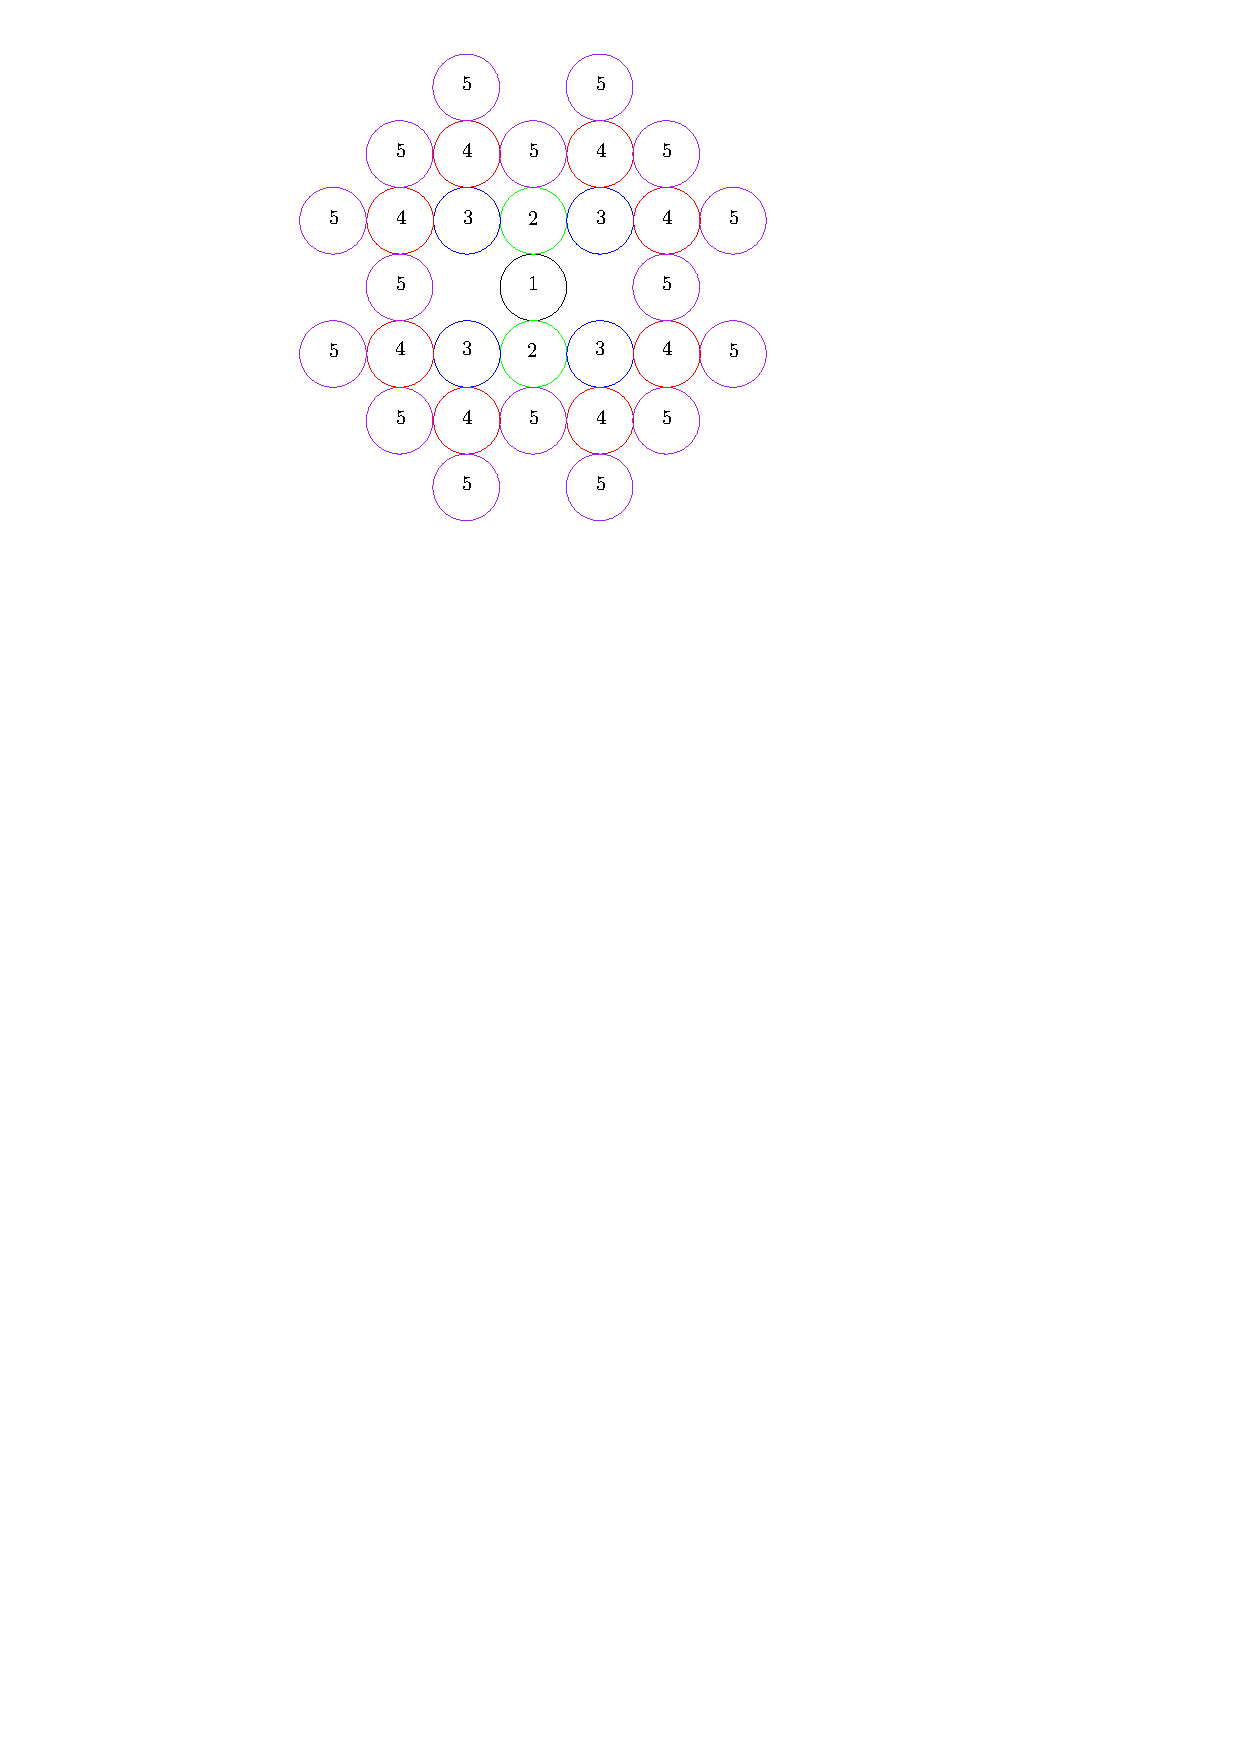
\includegraphics[width=\textwidth]{graphics/degree5arrangement.pdf}
	  \caption{A disk arrangement with five layers of disks}
	  \label{fig:circlePacking1-3}
  \end{subfigure}
\end{center} 
\caption{The gradual growth of disk arrangements by adding two kissing disks to each of the previously generated disks.  By continuing this arrangement growth, the space needed to contain the kissing disks will exceed the area containing the disk arrangements.}\label{fig:circlePacking-1}
\end{figure}
This is so frustrating to explain.  I understand it, I have trouble explaining it.  Then I'd like to show how this relates to our problem.